\chapter{Data Samples}

\section{BrilCalc command for B-Parking HLT path}\label{sec:PU}
The analysis uses B Parking datasets. Data was
collected during the 2018 portion of Run 2 and corresponds to an integrated luminosity of
 50~$\mathrm{fb}^{-1}$.

\begin{table}[htb!]
  \caption{Datasets used in the analysis}
  \begin{center}
    %\footnotesize
    %\scriptsize
    \begin{tabular}{l|l}\hline
      Data sample & Integrated Luminosity (pb$^-1$)\\
      \hline
      /ParkingBPH1/Run2018A-UL2018\_MiniAODv2-v1/MINIAODD  & 867.13 \\
      /ParkingBPH2/Run2018A-UL2018\_MiniAODv2-v1/MINIAODD  & 859.38 \\
      /ParkingBPH3/Run2018A-UL2018\_MiniAODv2-v1/MINIAODD  & 866.07 \\
      /ParkingBPH4/Run2018A-UL2018\_MiniAODv2-v1/MINIAODD  & 867.38 \\
      /ParkingBPH5/Run2018A-UL2018\_MiniAODv2-v1/MINIAODD  & 867.12 \\
      /ParkingBPH6/Run2018A-UL2018\_MiniAODv2-v1/MINIAODD  & 866.98 \\
      Total & 5194.1\\
      \hline
      /ParkingBPH1/Run2018B-UL2018\_MiniAODv2-v1/MINIAODD  & 882.57 \\
      /ParkingBPH2/Run2018B-UL2018\_MiniAODv2-v1/MINIAODD  & 881.37 \\
      /ParkingBPH3/Run2018B-UL2018\_MiniAODv2-v1/MINIAODD  & 882.31 \\
      /ParkingBPH4/Run2018B-UL2018\_MiniAODv2-v1/MINIAODD  & 882.32 \\
      /ParkingBPH5/Run2018B-UL2018\_MiniAODv2-v1/MINIAODD  & 882.30 \\
      /ParkingBPH6/Run2018B-UL2018\_MiniAODv2-v1/MINIAODD  & 399.63 \\
      Total & 4810.5\\
      \hline
      /ParkingBPH1/Run2018C-UL2018\_MiniAODv2-v1/MINIAODD  & 1171.8 \\
      /ParkingBPH2/Run2018C-UL2018\_MiniAODv2-v1/MINIAODD  & 1171.8 \\
      /ParkingBPH3/Run2018C-UL2018\_MiniAODv2-v1/MINIAODD  & 1168.2 \\
      /ParkingBPH4/Run2018C-UL2018\_MiniAODv2-v1/MINIAODD  & 1171.8 \\
      /ParkingBPH5/Run2018C-UL2018\_MiniAODv2-v1/MINIAODD  & 1165.3 \\
      Total & 5848.9\\
      \hline
      /ParkingBPH1/Run2018D-UL2018\_MiniAODv2-v1/MINIAODD  & 5640.4 \\
      /ParkingBPH2/Run2018D-UL2018\_MiniAODv2-v1/MINIAODD  & 5619.6 \\
      /ParkingBPH3/Run2018D-UL2018\_MiniAODv2-v1/MINIAODD  & 5634.3 \\
      /ParkingBPH4/Run2018D-UL2018\_MiniAODv2-v1/MINIAODD  & 0. \\
      /ParkingBPH5/Run2018D-UL2018\_MiniAODv2-v1/MINIAODD  & 5622.1 \\
      Total & 22516.4\\
      \hline
      ParkingBPH Total & 38369.9 \\
      \hline
    \end{tabular}
    \label{tab:datasample2018BPH}
  \end{center}
\end{table}


\begin{verbatim}
brilcalc lumi --byls --normtag 
/cvmfs/cms-bril.cern.ch/cms-lumi-pog/Normtags/normtag_PHYSICS.json 
-i processedLumis.json --hltpath HLT_Mu9_IP6_part0_v* -o output.csv
\end{verbatim}
Please note that we get luminosity for the specific BPH HLT path and save the output for pileupReCalc\_HLTpaths.py

\begin{verbatim}
pileupReCalc_HLTpaths.py -i output.csv 
--inputLumiJSON pileup_latest.txt -o My_HLT_corrected_PileupJSON.txt 
--runperiod Run2
\end{verbatim}

where, pileup\_latest.txt is from

\begin{verbatim}
/afs/cern.ch/cms/CAF/CMSCOMM/COMM_DQM/certification/Collisions18/
13TeV/PileUp/pileup_latest.txt
\end{verbatim}


Then, we substitute the usual pileup\_latest.txt to My\_HLT\_corrected\_PileupJSON.txt to obtain the PU distribution of data. 

\begin{verbatim}
pileupCalc.py -i processedLumis.json 
--inputLumiJSON My\_HLT\_corrected\_PileupJSON.txt  
--calcMode true --minBiasXsec 69200 --maxPileupBin 120 --numPileupBins 120 
MyDataPileupHistogram.root
\end{verbatim}

With histograms above, one can create a PUWeight histogram distribution for an era's specific HLT path with commands below.
\begin{verbatim}
PUdata->Scale(1./PUdata->Integral(0,-1));
PUmc->Scale(1./PUmc->Integral(0,-1));
PUdata->Divide(PUmc);
\end{verbatim}

\section{Monte Carlo Samples}

\subsection{Signal Model and Simulation}

The ggH production process (see Figure~\ref{fig:feynmanggH}) is generated at next-to-next-to-leading order (NNLO) and next-to-next-to-leading-log (NNLL) QCD and next-to-leading order (NLO) EW accuracies ~\cite{Heinemeyer:2013xd}.
The Higgs boson mass is set to 125GeV for all signal samples.
The cross sections, computed at NNLO+NNLL QCD and NLO EW accuracies and obtained from CERN Yellow Report 3,
are 4.414~$\mathrm{pb}$. The CMS detector response is modeled with GEANT4~\cite{Agostinelli:2002hh}.

\begin{figure}[h!]
  \caption{Leading Feynman diagrams for ggH production mode}
  \label{fig:feynmanggH}
  \centering
  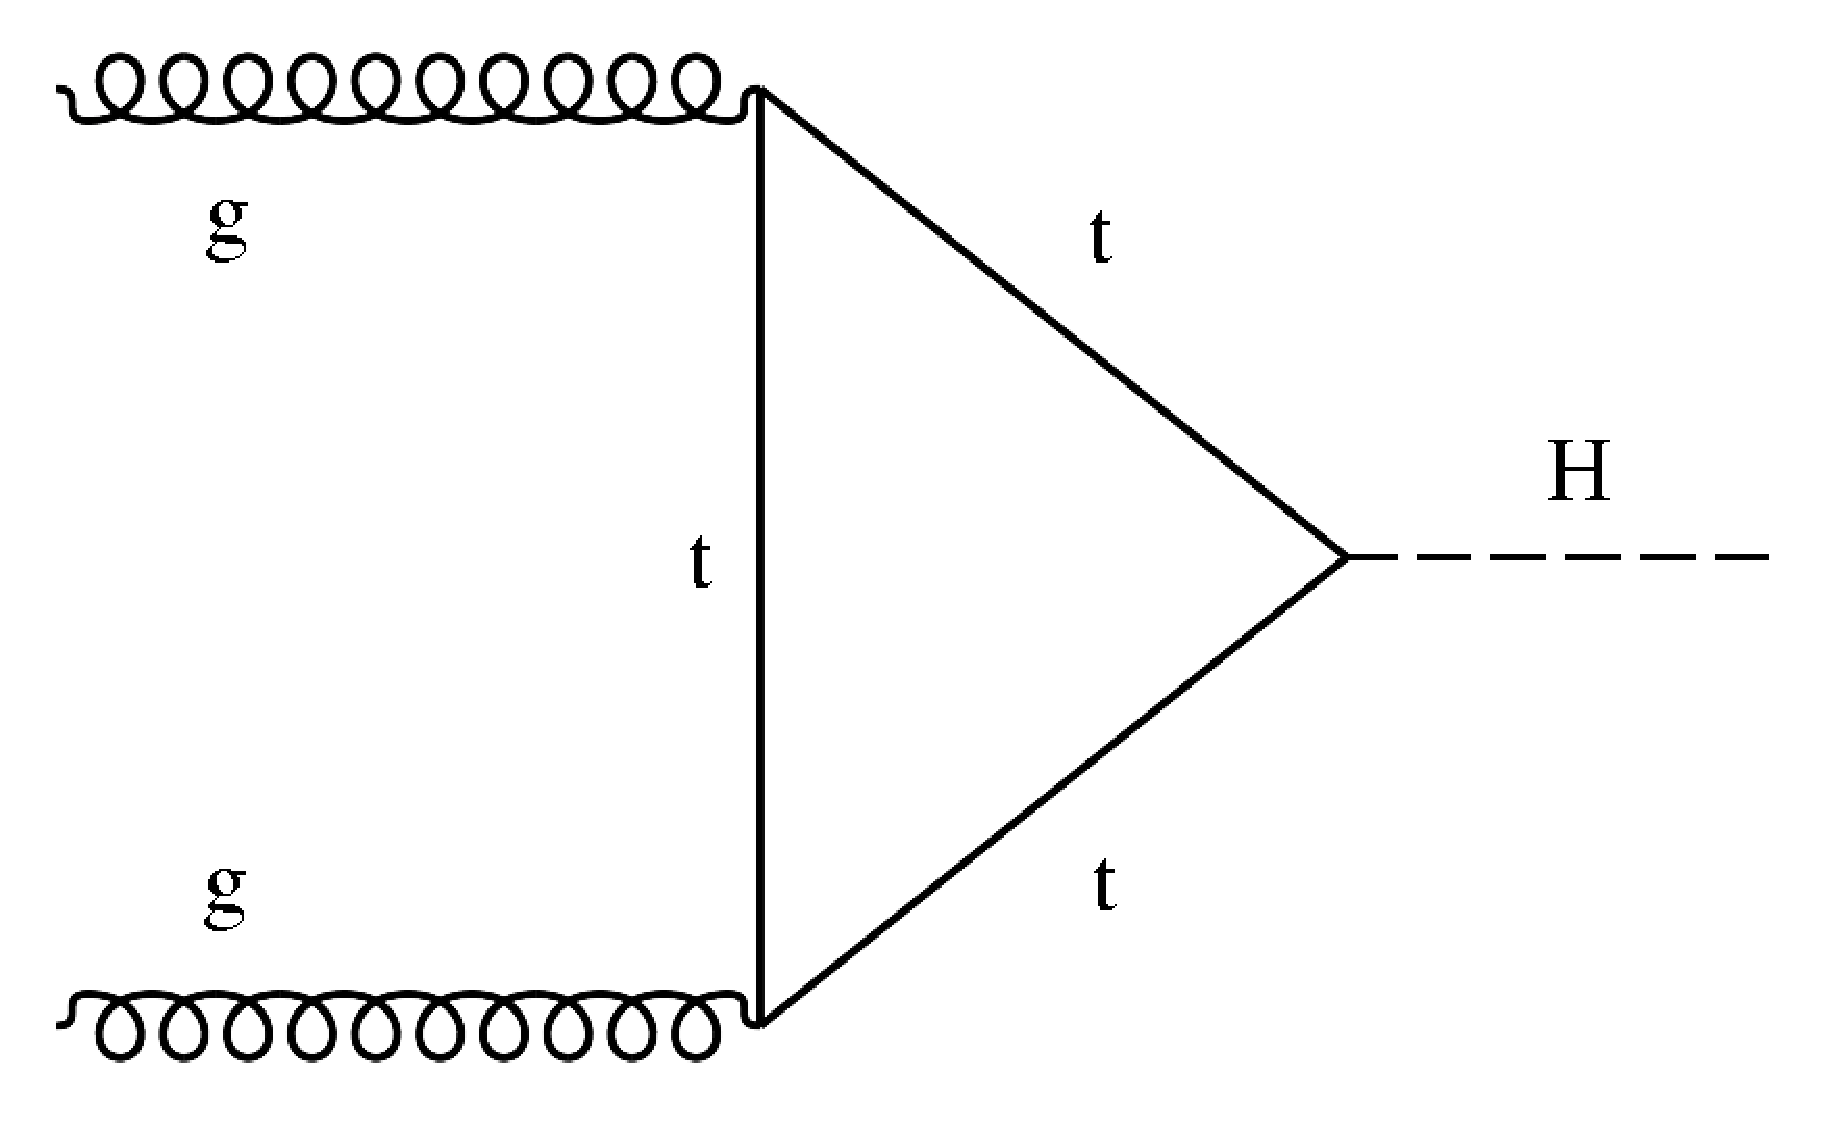
\includegraphics[width=0.47\linewidth]{figs/feynmanggH.pdf}

\end{figure}


%The Higgs boson decay to long-lived scalars is simulted using \PYTHIA v8.230~\cite{Sjostrand:2014zea}.
%The parton distribution functions used to produce all samples are the
%next-to-next-to-leading order (NNLO) NNPDF3.1 set~\cite{Ball:2017nwa}.
%For parton showering and hadronization, the matrix element generators are interfaced
%with \PYTHIA v8.230. For all samples, simulated additional pp interactions (pileup)
% are added to the hard-scattering process with the multiplicity distribution matched
% to the corresponding data-taking period (2016, 2017, 2018).
%The scalar is simulated as a generic scalar particle with a 100\% branching
%ratio to b-quarks (samples with scalar decays to light quarks and tau
%leptons also exist).
%We generate samples with varying scalar mass and lifetime, and include in this
%set of variations the
%benchmark points recommended by the LHCHXSWG~\cite{deFlorian:2016spz}.
Table~\ref{tab:sigsample} lists the signal Monte Carlo samples.
Due to lack of Ultra-Legacy campaign for the signal Monte Carlo, the analysis used the pre-Ultra-Legacy campaign signal Monte Carlo.
%%%%%%%%% %%%%%%%%%%%%%%%%%%%%%%%%%%%%%%%%%%%%%%%%%%%%%%%%%%%%%%%%%%%%%%%%%%%%%%%%
% The tables below are generated from lines like `python check_used.py | grep HToBB`
% using the script in LLDJstandalones/lists/ntuple
%%%%%%%%%%%%%%%%%%%%%%%%%%%%%%%%%%%%%%%%%%%%%%%%%%%%%%%%%%%%%%%%%%%%%%%%%%%%%%%%%%%%%%%%

\begin{table}[htb]
  %\caption{gg($h \rightarrow ss\rightarrow \tau\bar{\tau} \tau\bar{\tau}$) Signal Monte Carlo samples. Campaign is RunIIAutumn18MiniAOD-rp\_102X\_upgrade2018\_realistic\_v15-v1}
  \begin{center}
    %\footnotesize
    \scriptsize
    \begin{tabular}{l}\hline
      Sample \\
      \hline
      /ggH\_HToSSTo4Tau\_MH-125\_TuneCP5\_13TeV-powheg-pythia8/CAMPAIGN/MINIAODSIM\\
      \hline
      /ggH\_HToSSTo4Tau\_MH-125\_MS-55\_ctauS-1\_TuneCP5\_13TeV-powheg-pythia8/CAMPAIGN/MINIAODSIM\\
      /ggH\_HToSSTo4Tau\_MH-125\_MS-55\_ctauS-10\_TuneCP5\_13TeV-powheg-pythia8/CAMPAIGN/MINIAODSIM\\
      /ggH\_HToSSTo4Tau\_MH-125\_MS-55\_ctauS-100\_TuneCP5\_13TeV-powheg-pythia8/CAMPAIGN/MINIAODSIM\\
      /ggH\_HToSSTo4Tau\_MH-125\_MS-55\_ctauS-1000\_TuneCP5\_13TeV-powheg-pythia8/CAMPAIGN/MINIAODSIM\\
      /ggH\_HToSSTo4Tau\_MH-125\_MS-40\_ctauS-1\_TuneCP5\_13TeV-powheg-pythia8/CAMPAIGN/MINIAODSIM\\
      /ggH\_HToSSTo4Tau\_MH-125\_MS-40\_ctauS-10\_TuneCP5\_13TeV-powheg-pythia8/CAMPAIGN/MINIAODSIM\\
      /ggH\_HToSSTo4Tau\_MH-125\_MS-40\_ctauS-100\_TuneCP5\_13TeV-powheg-pythia8/CAMPAIGN/MINIAODSIM\\
      /ggH\_HToSSTo4Tau\_MH-125\_MS-40\_ctauS-1000\_TuneCP5\_13TeV-powheg-pythia8/CAMPAIGN/MINIAODSIM\\
      /ggH\_HToSSTo4Tau\_MH-125\_MS-15\_ctauS-1\_TuneCP5\_13TeV-powheg-pythia8/CAMPAIGN/MINIAODSIM\\
      /ggH\_HToSSTo4Tau\_MH-125\_MS-15\_ctauS-10\_TuneCP5\_13TeV-powheg-pythia8/CAMPAIGN/MINIAODSIM\\
      /ggH\_HToSSTo4Tau\_MH-125\_MS-15\_ctauS-100\_TuneCP5\_13TeV-powheg-pythia8/CAMPAIGN/MINIAODSIM\\
      /ggH\_HToSSTo4Tau\_MH-125\_MS-15\_ctauS-1000\_TuneCP5\_13TeV-powheg-pythia8/CAMPAIGN/MINIAODSIM\\
      /ggH\_HToSSTo4Tau\_MH-125\_MS-7\_ctauS-1\_TuneCP5\_13TeV-powheg-pythia8/CAMPAIGN/MINIAODSIM\\
      /ggH\_HToSSTo4Tau\_MH-125\_MS-7\_ctauS-10\_TuneCP5\_13TeV-powheg-pythia8/CAMPAIGN/MINIAODSIM\\
      /ggH\_HToSSTo4Tau\_MH-125\_MS-7\_ctauS-100\_TuneCP5\_13TeV-powheg-pythia8/CAMPAIGN/MINIAODSIM\\
      /ggH\_HToSSTo4Tau\_MH-125\_MS-7\_ctauS-1000\_TuneCP5\_13TeV-powheg-pythia8/CAMPAIGN/MINIAODSIM\\
      \hline
    \end{tabular}
    \label{tab:sigsample}
  \end{center}
  \caption{CAMPAIGN:RunIIAutumn18MiniAOD-rp\_102X\_upgrade2018\_realistic\_v15-v1}
\end{table}




%An example \PYTHIA v8.230 fragment for the Higgs decay to scalars (scalars) and their subsequent decay to tau leptons is given below.
%In this example the mass of the scalar is 15GeV and its lifetime (c$\tau$) is 10,000mm.
%\begin{verbatim}
%  '9000006:all = sk skbar 0 0 0 15 1.9732e-17 1.0 75.0 10000',
%  '9000006:oneChannel = 1  1.0 101  15 -15',
%  '9000006:mayDecay = on',
%  '9000006:isResonance = on',
%  '25:m0 = 125.0',
%  '25:onMode = off',
%  '25:addChannel = 1 0.000000001 101 9000006 -9000006',
%  '25:onIfMatch = 9000006 -9000006',
%  '9000006:onMode = off',
%  '9000006:onIfAny = 5',
%\end{verbatim}



\subsection{Background Monte Carlo}
All samples were processed as recommended in the PPD Run2 Analysis Guideline~\cite{pdmv}.
All background Monte Carlo samples have been completely produced in the Ultra-Legacy campaign as well.
Thus, the analysis used the Ultra-Legacy campaign background Monte Carlo.
The asterick mark denotes the campaign abbreviation, RunIISummer20UL18MiniAODv2-106X\_upgrade2018\_realistic\_v16\_L1v1.
Tables~\ref{tab:QCDsample}-\ref{tab:18samplesummary} summarizes the background Monte Carlo used in this analysis.

%%%%%%%%%%%%%%%%%%%%%%%%%%
%%%%%%%%%2018%%%%%%%%%%%%%
%%%%%%%%%%%%%%%%%%%%%%%%%%
\begin{table}[htb]
  \caption{QCD MuEnriched Pt5 background Monte Carlo samples}
  \begin{center}
    \footnotesize
    %\scriptsize
    \begin{tabular}{l}\hline
      Sample \\
      \hline
      /QCD\_Pt-15to20\_MuEnrichedPt5\_TuneCP5\_13TeV\_pythia8/*-v3/MINIAODSIM \\
      /QCD\_Pt-20to30\_MuEnrichedPt5\_TuneCP5\_13TeV\_pythia8/*-v4/MINIAODSIM \\
      /QCD\_Pt-30to50\_MuEnrichedPt5\_TuneCP5\_13TeV\_pythia8/*-v3/MINIAODSIM \\
      /QCD\_Pt-50to80\_MuEnrichedPt5\_TuneCP5\_13TeV\_pythia8/*-v3/MINIAODSIM \\
      /QCD\_Pt-80to120\_MuEnrichedPt5\_TuneCP5\_13TeV\_pythia8/*\_ext1-v2/MINIAODSIM \\
      /QCD\_Pt-120to170\_MuEnrichedPt5\_TuneCP5\_13TeV\_pythia8/*\_ext1-v2/MINIAODSIM \\
      /QCD\_Pt-170to300\_MuEnrichedPt5\_TuneCP5\_13TeV\_pythia8/*-v3/MINIAODSIM \\
      /QCD\_Pt-300to470\_MuEnrichedPt5\_TuneCP5\_13TeV\_pythia8/*\_ext3-v1/MINIAODSIM \\
      /QCD\_Pt-470to600\_MuEnrichedPt5\_TuneCP5\_13TeV\_pythia8/*\_ext1-v2/MINIAODSIM \\
      /QCD\_Pt-600to800\_MuEnrichedPt5\_TuneCP5\_13TeV\_pythia8/*-v1/MINIAODSIM \\
      /QCD\_Pt-800to1000\_MuEnrichedPt5\_TuneCP5\_13TeV\_pythia8/*\_ext3-v2/MINIAODSIM \\
      /QCD\_Pt-1000toInf\_MuEnrichedPt5\_TuneCP5\_13TeV\_pythia8/*-v1/MINIAODSIM \\
      \hline
    \end{tabular}
    \label{tab:QCDsample}
  \end{center}
\end{table}
a


\begin{table}[htb]
  \caption{W,Z,H boson background Monte Carlo samples}
  \begin{center}
    \footnotesize
    \begin{tabular}{l}\hline
      Sample \\
      \hline
      /DYJetsToLL\_M-50\_TuneCP5\_13TeV-madgraphMLM-pythia8/*-v1/MINIAODSIM \\
      \hline
      /WJetsToLNu\_M-50\_TuneCP5\_13TeV-madgraphMLM-pythia8/*-v2/MINIAODSIM \\
      \hline
      /WW\_M-50\_TuneCP5\_13TeV-madgraphMLM-pythia8/*-v2/MINIAODSIM \\
      /WZ\_M-50\_TuneCP5\_13TeV-madgraphMLM-pythia8/*-v3/MINIAODSIM \\
      /ZZ\_M-50\_TuneCP5\_13TeV-madgraphMLM-pythia8/*-v2/MINIAODSIM \\
      \hline
      /GluGluHToBB\_M125\_13TeV\_amcatnloFXFX\_pythia8/*-v1/MINIAODSIM \\
      \hline
    \end{tabular}
    \label{tab:wzsample}
  \end{center}
\end{table}


\begin{table}[htb]
  \caption{Top background Monte Carlo samples}
  \begin{center}
    \footnotesize
    \begin{tabular}{l}\hline
      Sample \\
      \hline
      /TTJets\_TuneCP5\_13TeV-madgraphMLM-pythia8/*-v1/MINIAODSIM \\
      \hline
      /ST\_s-channel\_4f\_hadronicDecays\_TuneCP5\_13TeV-madgraph-pythia8/*\_ext1-v1/MINIAODSIM \\
      /ST\_t-channel\_top\_5f\_TuneCP5\_13TeV-powheg-pythia8/*-v1/MINIAODSIM \\
      /ST\_t-channel\_antitop\_5f\_TuneCP5\_13TeV-powheg-pythia8/*-v1/MINIAODSIM \\
      /ST\_tW\_antitop\_5f\_inclusiveDecays\_TuneCP5\_13TeV-powheg-pythia8/*\_ext1-v1/MINIAODSIM \\
      /ST\_tW\_top\_5f\_inclusiveDecays\_TuneCP5\_13TeV-powheg-pythia8/*\_ext1-v1/MINIAODSIM \\
      \hline
    \end{tabular}
    \label{tab:topsample}
  \end{center}
\end{table}


\begin{table}[htb]
  \caption{Monte Carlo sample summary}
  \begin{center}
    \footnotesize
    %\scriptsize
    \begin{tabular}{l}\hline
      Sample \\
      \hline
      /QCD\_Pt-15to20\_MuEnrichedPt5\_TuneCP5\_13TeV\_pythia8/*-v3/MINIAODSIM \\
      /QCD\_Pt-20to30\_MuEnrichedPt5\_TuneCP5\_13TeV\_pythia8/*-v4/MINIAODSIM \\
      /QCD\_Pt-30to50\_MuEnrichedPt5\_TuneCP5\_13TeV\_pythia8/*-v3/MINIAODSIM \\
      /QCD\_Pt-50to80\_MuEnrichedPt5\_TuneCP5\_13TeV\_pythia8/*-v3/MINIAODSIM \\
      /QCD\_Pt-80to120\_MuEnrichedPt5\_TuneCP5\_13TeV\_pythia8/*\_ext1-v2/MINIAODSIM \\
      /QCD\_Pt-120to170\_MuEnrichedPt5\_TuneCP5\_13TeV\_pythia8/*\_ext1-v2/MINIAODSIM \\
      /QCD\_Pt-170to300\_MuEnrichedPt5\_TuneCP5\_13TeV\_pythia8/*-v3/MINIAODSIM \\
      /QCD\_Pt-300to470\_MuEnrichedPt5\_TuneCP5\_13TeV\_pythia8/*\_ext3-v1/MINIAODSIM \\
      /QCD\_Pt-470to600\_MuEnrichedPt5\_TuneCP5\_13TeV\_pythia8/*\_ext1-v2/MINIAODSIM \\
      /QCD\_Pt-600to800\_MuEnrichedPt5\_TuneCP5\_13TeV\_pythia8/*-v1/MINIAODSIM \\
      /QCD\_Pt-800to1000\_MuEnrichedPt5\_TuneCP5\_13TeV\_pythia8/*\_ext3-v2/MINIAODSIM \\
      /QCD\_Pt-1000toInf\_MuEnrichedPt5\_TuneCP5\_13TeV\_pythia8/*-v1/MINIAODSIM \\
      /DYJetsToLL\_M-50\_TuneCP5\_13TeV-madgraphMLM-pythia8/*-v1/MINIAODSIM \\
      /WJetsToLNu\_M-50\_TuneCP5\_13TeV-madgraphMLM-pythia8/*-v2/MINIAODSIM \\
      /WW\_M-50\_TuneCP5\_13TeV-madgraphMLM-pythia8/*-v2/MINIAODSIM \\
      /WZ\_M-50\_TuneCP5\_13TeV-madgraphMLM-pythia8/*-v3/MINIAODSIM \\
      /ZZ\_M-50\_TuneCP5\_13TeV-madgraphMLM-pythia8/*-v2/MINIAODSIM \\
      /GluGluHToBB\_M125\_13TeV\_amcatnloFXFX\_pythia8/*-v1/MINIAODSIM \\
      /TTJets\_TuneCP5\_13TeV-madgraphMLM-pythia8/*-v1/MINIAODSIM \\
      /ST\_s-channel\_4f\_hadronicDecays\_TuneCP5\_13TeV-madgraph-pythia8/*\_ext1-v1/MINIAODSIM \\
      /ST\_t-channel\_top\_5f\_TuneCP5\_13TeV-powheg-pythia8/*-v1/MINIAODSIM \\
      /ST\_t-channel\_antitop\_5f\_TuneCP5\_13TeV-powheg-pythia8/*-v1/MINIAODSIM \\
      /ST\_tW\_antitop\_5f\_inclusiveDecays\_TuneCP5\_13TeV-powheg-pythia8/*\_ext1-v1/MINIAODSIM \\
      /ST\_tW\_top\_5f\_inclusiveDecays\_TuneCP5\_13TeV-powheg-pythia8/*\_ext1-v1/MINIAODSIM \\
      \hline
      /ggH\_HToSSTo4Tau\_MH-125\_TuneCP5\_13TeV-powheg-pythia8/*-v1/MINIAODSIM\\
      \hline
    \end{tabular}
    \label{tab:18samplesummary}
  \end{center}
\end{table}

\chapter{Machine Learning Training Variable}

Loss, Accuracy, validation loss, validation accuracy, and AUC values are recorded for the number of epochs run.

\begin{table}[htb]
\caption{Tensorflow information}
\begin{center}
\begin{tabular}{r|l|l|l|l|l}\hline
Epoch &  loss & acc &  val\_loss & val\_acc & AUC\\
\hline
100& 0.2161 & 0.9074 & 0.2469 & 0.8942 & 0.9387\\
150& 0.2039 & 0.9120 & 0.2393 & 0.8983 & 0.9414\\
200& 0.1934 & 0.9151 & 0.2523 & 0.8953 & 0.9408\\
250& 0.1977 & 0.9144 & 0.2459 & 0.8982 & 0.9399\\
300& 0.1738 & 0.9272 & 0.2573 & 0.8977 & 0.9387\\
350& 0.1607 & 0.9332 & 0.2693 & 0.8934 & 0.9403\\
400& 0.1459 & 0.9387 & 0.2823 & 0.8970 & 0.9394\\
\hline
\end{tabular}
\label{tab:Epoch Training}
\end{center}
\end{table}

Loss, Accuracy, and AUC values are recorded for the combination of signal point and the background process.
\begin{table}[htb]
\caption{Tensorflow information}
\begin{center}
\begin{tabular}{r|l|l|l|l}\hline
Signal & Background & Loss & Accuracy & AUC\\
\hline
ggH\_HToSSTo4Tau\_MH-125\_MS-7\_ctauS-10& QCDMuEnrichedPt5\_Pt20-30 & 0.1852 & 0.9244 & 0.9696\\
& QCDMuEnrichedPt5\_Pt470-600 & 0.1597 & 0.9361 & 0.9727\\
& TTJets & 0.1681 & 0.9320 & 0.9680\\
\hline
ggH\_HToSSTo4Tau\_MH-125\_MS-15\_ctauS-10& QCDMuEnrichedPt5\_Pt20-30 & 0.2133 & 0.9093 & 0.9598\\
& QCDMuEnrichedPt5\_Pt470-600 & 0.1687 & 0.9306 & 0.9679\\
& TTJets & 0.1838 & 0.9242 & 0.9610\\
\hline
ggH\_HToSSTo4Tau\_MH-125\_MS-15\_ctauS-100& QCDMuEnrichedPt5\_Pt20-30 & 0.0747 & 0.9755 & 0.9791\\
& QCDMuEnrichedPt5\_Pt470-600 & 0.1596 & 0.9361 & 0.9727\\
& TTJets & 0.1681 & 0.9320 & 0.9680\\
\hline
ggH\_HToSSTo4Tau\_MH-125\_MS-40\_ctauS-100& QCDMuEnrichedPt5\_Pt20-30 & 0.1898 & 0.9209 & 0.9695\\
& QCDMuEnrichedPt5\_Pt470-600 & 0.1765 & 0.9275 & 0.9698\\
& TTJets & 0.1576 & 0.9379 & 0.9705\\
\hline
ggH\_HToSSTo4Tau\_MH-125\_MS-55\_ctauS-100& QCDMuEnrichedPt5\_Pt20-30 & 0.1898 & 0.9227 & 0.9635\\
& QCDMuEnrichedPt5\_Pt470-600 & 0.1480 & 0.9399 & 0.9674\\
& TTJets & 0.1433 & 0.9450 & 0.9706\\
\hline
\end{tabular}
\label{tab:Epoch Training}
\end{center}
\end{table}


